\section{Results}
\begin{doublespacing}
In this study, heat conduction simulations were used to study the impact of overall heat transfer coefficient in the presence of Xenon bubble in the intragranular region. Grain boundary resistance and the influence of intergranular fission is not included in this calculation. This simulation is design to see the impact on heat transfer due to the formation of Gas Bubble Superlattice. Bubble superlattice formation inside U-Mo fuel stabilizes the fuel swelling behavior but heavily impacts the heat transfer capability~\cite{burkes2015thermal}. This might be due to Xenon's very low thermal conductivity. Thermal properties of Xenon was also considered in this work. Xenon's thermal conductivity is a function of both temperature and pressure~\cite{rabinovich1987thermophysical}. Since the size of the bubble changes with the burnup and fission density, thermal conductivity of the bubble also changes~\cite{miller2012advantages}. Pressure inside the bubble is highly depend on the curvature of the bubble. The reults is plotted in figure~\ref{fig_result}. As it can be seen from the plot that thermal conductivity of U-10Mo drops with the presence of the Xenon bubble. And with the increase of the Xenon bubble's size it also decreases. The result is also compared with Maxwell-Eucken equation~\cite{maxwell1881treatise} and with Hashin and Strikman~\cite{hashin1962variational}. In figure~\ref{fig_compare} the comparison is showed. 

\begin{figure}[H]
\centering
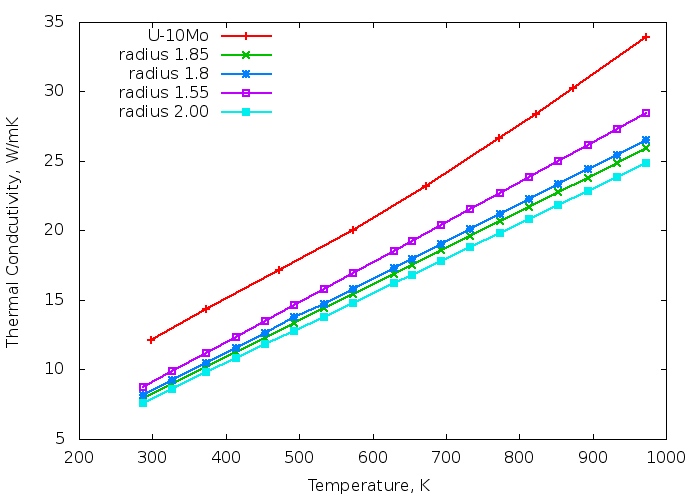
\includegraphics[scale=0.5]{result_Xe_U-10Mo.png}
\caption{Comparison between the thermal conductivity of U-10Mo and the inclusion of Xe bubble of different sizes}
\label{fig_result}
\end{figure}

FEM calculations were performed on \ref{fcc_mesh} in order to calculate the thermal flux and the thermal conductivity in 2D. Since thermal conductivity of Xenon is a function of both temperature and pressure, six different pressure has been chosen to represend the conductivity (Figure~\ref{fig_Xe_K}). Eventhough the dependence of thermal conductivity is evident, the results show no change in the overall thermal conductivity in the fuel. Pressure in the bubble is significantly higher than the 1000 bar in some situation~\cite{xiao2015atomistic}. The increased pressure inside the bubble creates another probability of having phase change from gas to solid~\cite{zheng2014thermodynamics}. So the resluts show that with the increased pressure inside the Xenon bubble, the overall thermal conductivity has a very negligible effect. 


\begin{figure}[H]
	\centering
	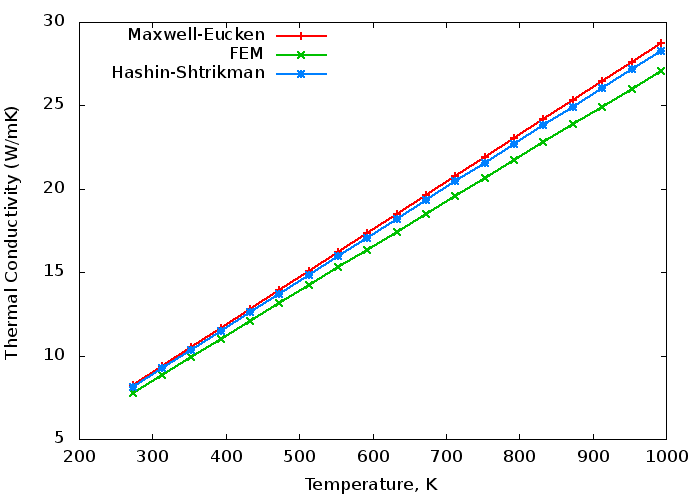
\includegraphics[scale=0.5]{theory_compare.png}
	\caption{Comparison of predicted thermal conductivity of U-10Mo with Xenon bubble against the Maxwell-Eucken and Hashin and Shtrikman }
	\label{fig_compare}
	\end{figure}


\begin{figure}[H]
	\centering
	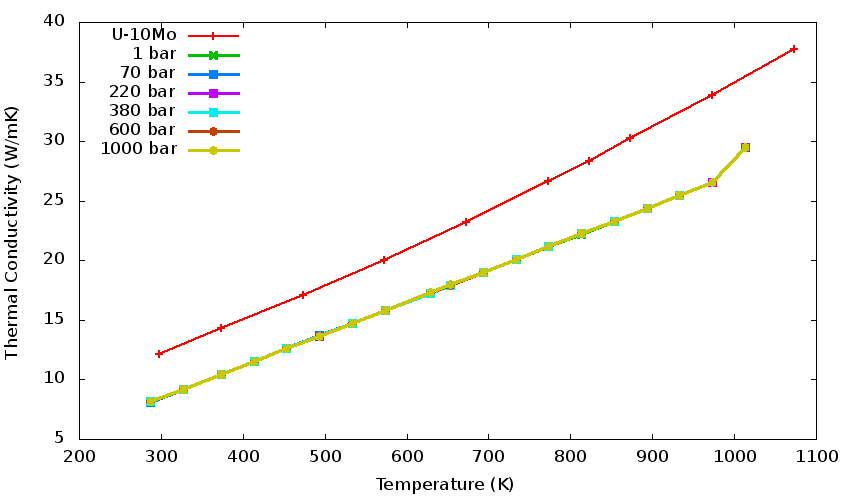
\includegraphics[scale=0.5]{press_eff_k.png}
	\caption{Over all thermal conductivity U-10Mo using thermal conductivity of Xenon of several pressure}
	\label{fig_press_K}
	
\end{figure}




\end{doublespacing}
